\chapter{Prototypes et résultats de tests préparatoires}


\section{Modèle}
\subsection{Prototype}
Aucune modification n'a été apporté au prototype papier. Nous avons donc décidé d'implémenter ce prototype (Figure 5.1.).



\subsection{Tests envisagés}
\begin{itemize}
  \item Tests généraux liés à l'implémentation d'une classe (constructeur, getters/setters, etc...).
  \item  Tests sur l'intégration du réseau de neurones au sein de la créature.\\

\end{itemize}


\section{Réseau de neurones}
\subsection{Prototype}
\begin{figure}[H]
    \centering
    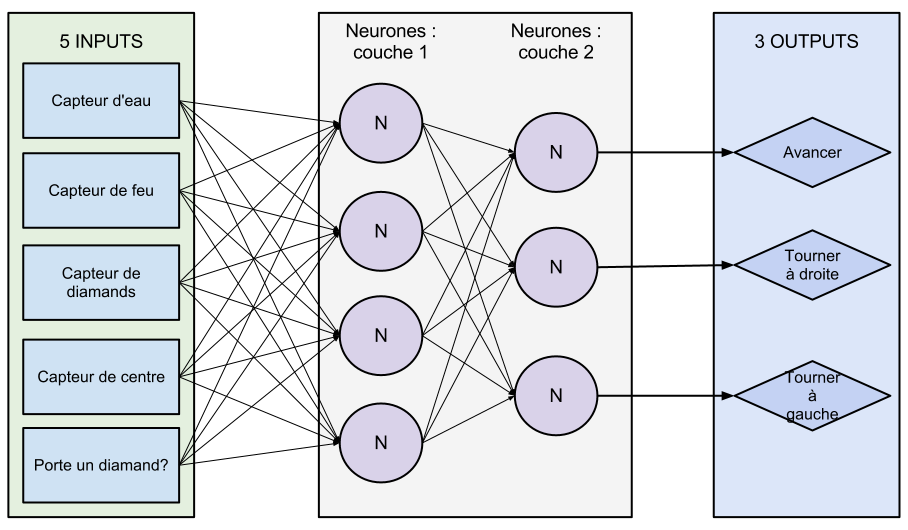
\includegraphics[width=1\textwidth]{./pictures/notre_reseau_neurones.png}
    \caption{Réseau de neurones}
\end{figure}


\subsection{Tests envisagés}

\begin{itemize}
  \item Tests pour déterminer le nombres de neurones et de couches qui seront utilisés.
  \item Tests pour choisir l'odre de grandeur des valeurs à atteindre afin d'exciter un neurone.
  \item Tests pour implémenter une généricité efficace (tests avec différents nombres et types d'entrées). \\

\end{itemize}

\section{Algorithme génétique}

\subsection{Prototype}
\begin{figure}[H]
    \centering
    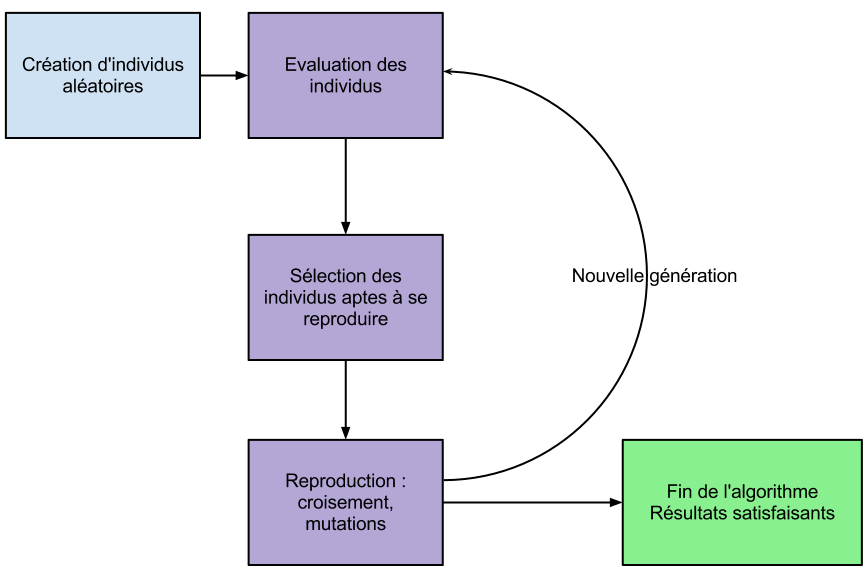
\includegraphics[width=1\textwidth]{./pictures/algo_creatures.png}
    \caption{Algo }
\end{figure}


\subsection{Tests envisagés}
\begin{itemize}
  \item Tests des différentes techniques de sélection (par rang, par tournois, etc...).
  \item Tests des différentes techniques de croisement et reproduction.
  \item Tests liés aux pourcentages d'individus sur lesquels appliquer les techniques (par exemple on décide d'effectuer une sélection par rang sur 60\% des individus et par tournoi sur 40\%). \\

\end{itemize}

\section{Interface graphique}
\subsection{Prototype}
\begin{figure}[H]
    \centering
    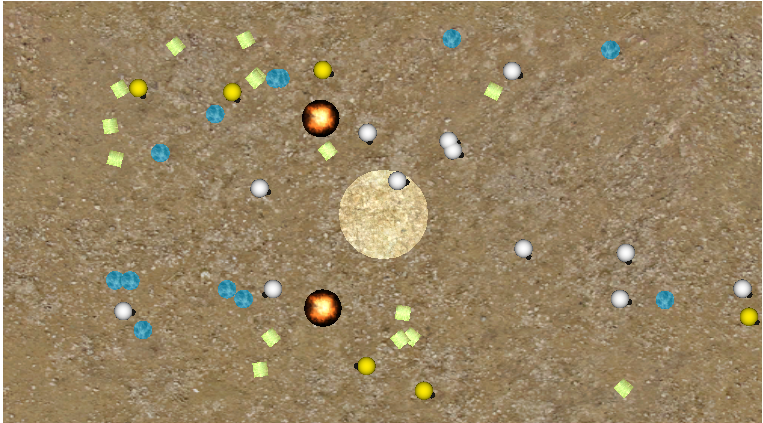
\includegraphics[width=1\textwidth]{./pictures/unity.png}
    \caption{Unity}
\end{figure}

\subsection{Tests envisagés}
Plusieurs tests à différents niveaux devront être effectués:
\begin{itemize}
  \item Gestion des collisions entre les créatures et les éléments de l'environnement.
 \item Affectation des inputs de la créature, voir si elle détecte bien les différents éléments (champs de vision et Raycasts).
 \item Rendu des outputs (déplacements) de la créature.
 \item Différents tests liés à une interface graphique.
\end{itemize}
\clearpage
